\chapter{Blinking Eye Simulation}

\section{Introduction}

The tear film is a very thin layer of liquid film on the ocular surface spread through blinking. It serves several vital functions including protecting the the ocular surface with moister, transporting waste, as well as providing a smooth ocular surface; within each blink cycle, a tear film that is functioning properly will maintain a balance between tear secretion and loss. \cite{holly1977tear}.

	Dry eye syndrome (DES) is a collection of symptoms that include (but or not limited too) blurred vision, burning, foreign body sensation, as well as tearing and inflammation of the ocular surface. An estimated 4.91 million Americans suffer from DES (according to a study from 2007) \cite{bron2007methodologies}. A malfunctioning or deficient tear film is thought to be a cause of DES \cite{nelson2011international}, causing the ocular tear film comunity to take interest in the function of the tear film \cite{johnson2004changes} as well as the connection between tear film volume, evaporation and break up with DES \cite{bron2007methodologies}.
	
\begin{figure}
  \centering
  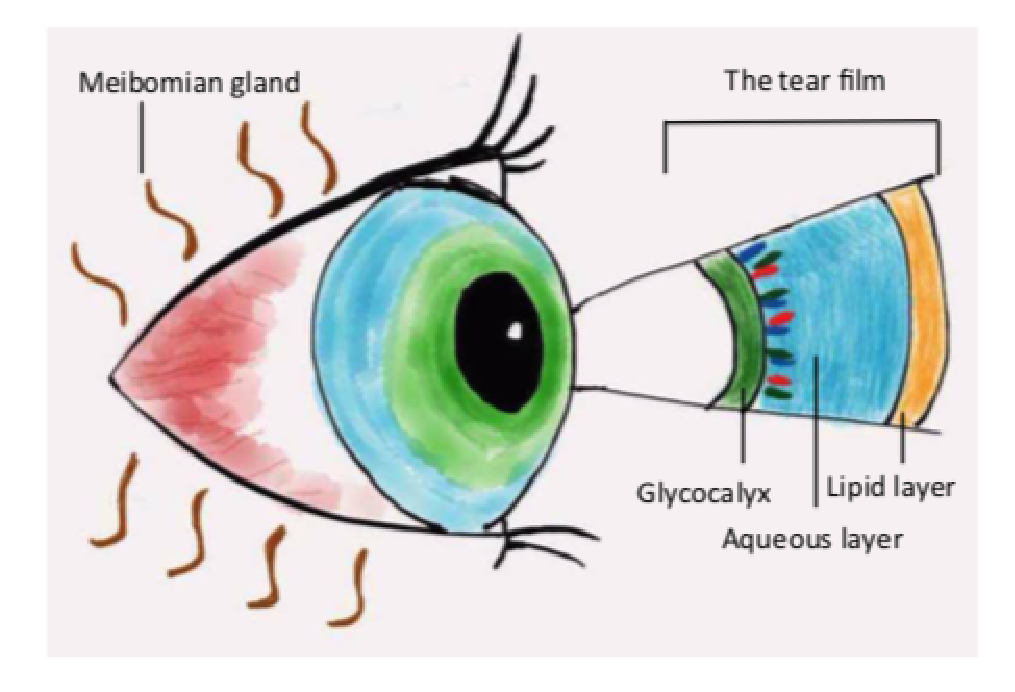
\includegraphics[scale=0.6]{Chapter4/eye_model.eps}
  \caption{Illustration of tear film with labeled layers.}
  \label{eye_levels}
\end{figure}

	The tear film is composed of three layers, as shown in Figure~\ref{eye_levels}. The anterior surface in contact with the air is an oily lipid layer which helps reduce evaporation \cite{norn1979semiquantitative,mishima1961oily}. The middle aqueous layer is composed mostly of water, and serves to lubricate the eye, move particles as well as prevent infections. On the surface of the cornea sits the Glycocalyx layer, a a forest of proteins that moisturize the corneal surface by attracting water \cite{gipson2004distribution}. 
	
	A key component in simulating the tear film is developing numerical techniques that accommodate for realistic features of the underlying model. In 2008, Maki used the \textit{overset grid} method to study the effects of the tear film under reflex tearing \cite{maki2008overset}. In an overset grid method, A PDE is discretized and solved on a composite of grids to handle complex geometries and localized features of the function, where the overlapping grids are coupled through interpolation. Maki used fine boundary grids near the upper and lower eyelids in a 1D model to capture localized capillary thinning \cite{maki2008overset}.
	
	Maki extend this technique in 2D allowing for numerical simulations an a realistic open eye domain \cite{maki2010tear,maki2010tear2}. Using the Overature framework from Lawrence Livermore National Laboratory, she was able to generate a set of grids adopted to the geometry of the eye \cite{chesshire1990composite}; an example of this discritization can be seen in Figure~\ref{overature_eye}. It was found that the geometry, along side a tear film thickness boundary condition, produces stronger capillary action in the vicinities of the nasal and temporal canthi \cite{maki2010tear}. Maki later incorporated flux boundary conditions that depended both on space and time. She explored no flux boundary conditions on a realistic eye shaped domain, as well as non zero flux conditions that incorporated the influx from the lacrimal gland and puncta drainage \cite{maki2010tear2}. Li built on top these models to study the dynamics of osmolarity within the tear film \cite{li2012model,li2015computed}.
	
\begin{figure}
	\centering
	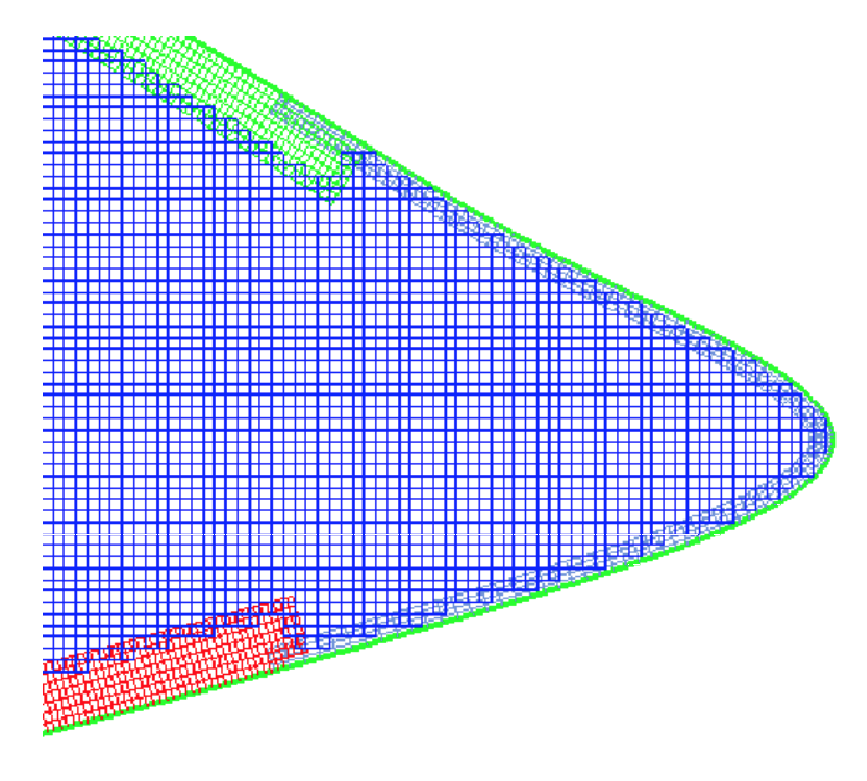
\includegraphics[scale=0.6]{Chapter4/overature_eye}
	\caption{Example of overlapping finite difference grids using Overature. }
	\label{overature_eye}
\end{figure}

Deng and Driscoll extended the one dimensional model of Braun and Li \cite{li2012model} to incorporate a moving boundary to simulate a blink, where Chebyshev polynomial approximations were used in the discretization. Through this new model, it was observed that blinking has an effect on the cooling of the tear film \cite{deng2013model,deng2014heat}. Driscoll and Braun then extended these techniques to simulate parabolic flow on an eye shaped domain \cite{driscoll2018simulation}. As a start, they found numerical solutions for the model
\begin{equation}
\label{driscollPDE}
h_t + \nabla \cdot \vect{q} (h,h_x,h_y)=0, \quad (x,y) \in \mathcal{E}(t)
\end{equation}
where $h$ is the prescribed film thickness and $\vect{q}$ is a known flux function. The domain $\mathcal{E}(t)$ is a realistic eye domain that changes with time, visualized in Figure~\ref{driscoll_eye} and defined in the following section. In particular they examined a second order thin film analog where
\begin{equation}
\label{thin_film_analog}
\vect{q} = -(A-B h^{-3})\nabla h
\end{equation}
for constants $A$ and $B$ \cite{driscoll2018simulation}. Numerically the PDE is discritized with a Chebyshev polynomial tensor product approximation. In the case of the second order thin film analog with flux (\ref{thin_film_analog}), this led to a solution that was accurate to at least five digits.

In this chapter, we seek to extend this method to solve a fourth order tear film model in a DAE where the pressure is solved algebraically. In order to meet the needed computational demands we will use our new preconditioned techniques to solve this problem. In the following sections, we describe the fourth order tear film model, as well as briefly review how the blinking eye domain $\mathcal{E}(t)$ is transformed from the $[-1,1]^2$. We conclude with a numerical study of our method on the PDE.


\begin{figure}
  \centering
  \includegraphics[scale=0.6]{Chapter4/different_domains}
  \caption{Plot of the subdomains used in \cite{driscoll2018simulation}, where $\mathcal{C}$, $\mathcal{R}(t)$, $\mathcal{E}(t)$ domains are the square, infinite strip and eye shaped domain. The mappings between the domains are explained in the following section.}
  \label{driscoll_eye}
\end{figure}
	
\section{model description}

We numerically solve for the height of the tear film $h(x,y)$ and pressure $p(x,y)$ with the model (\ref{driscollPDE}) using flux $\bm{q} =  \frac{h^3}{3} \nabla p$ where the pressure is solved algebraically, i.e.
\begin{align}
\begin{aligned}
h_t &= - \nabla \cdot \lp \frac{h^3}{3} \nabla p \rp, \\
p &= - \ps \nabla^2 h - \pa h^{-3}.
\end{aligned} \quad (x,y) \in \mathcal{E}(t)
\label{the_pde}
\end{align}
On the boundary we enforce a Dirichlet condition for $h$, as well as flux conditions on $p$ (with prescribed supply and drainage of fluid) that ensure that the volume of $h$ on $\mathcal{E}(t)$ is conserved over a blink cycle.
%\begin{align}
%\begin{aligned}
%h &= h_{c}, \\
%\bm{n} \cdot \bm{q} &=0
%\end{aligned} \quad (x,y) \in \partial \mathcal{E}(t)
%\label{boundary_conds}
%\end{align}

The domain $\mathcal{E}(t)$ is determined by a pair of two dimensional transforms. First a fixed square $\mathcal{C}=[-1,1]^2$ is mapped to an infinite strip $\mathcal{R}(t)$ by
\begin{align}
\mathcal{R}(t) = \{(x,y):|y|<\lambda(t)\}	
\end{align}
where $-1<\lambda(t)<1$ is a prescribed function satisfying $\lambda(0)=1$ (corresponding to a fully open eye). In this chapter, we use the realistic blink motion from \cite{deng2014heat}. For $(\hat{x},\hat{y}) \in \mathcal{C}$, $\mathcal{C}$ is mapped to $\mathcal{R}(t)$ via
\begin{align}
	g_x(\hat{x}) = \frac{\gamma \hat{x}}{\alpha^2 - \hat{x}}, \quad g_y(\hat{y}) = \frac{1}{2} (\hat{y}+1)(\lambda(t)+1)-1
\end{align}
for some $\gamma>0$ and $\alpha \geq 1$.


The domain $\mathcal{E}(t)$ is the image of $\mathcal{R}(t)$ under the conformal map
\begin{align}
f(z) = \tanh(z)	
\end{align}
i.e.,
\begin{align}
\mathcal{E}(t) = \{\operatorname{Re}(f(x+iy)),\operatorname{Im}(f(x+iy))|(x,y) \in \mathcal{R}(t)  \}.
\end{align}

If we define $\hat{\nabla}$ to be the gradient in terms of $(\hat{x},\hat{y})$ then
%\begin{align}
%\hat{\nabla} = \frac{\lp \cos(g_y(\hat{y}))+\cosh(g_x(\hat{x})) \rp^2}{1+\cos(g_y(\hat{y}))\cosh(g_x(\hat{x}))} \lp \frac{(\hat{x}^2+\alpha^2)\gamma}{(\hat{x}^2-\alpha^2)^2} \frac{d}{d \hat{x}}, \frac{2}{1+\lambda(t)} \frac{d}{d \hat{y}} \rp.
%\end{align}

\begin{align}
\hat{\nabla} = \frac{1}{|f'(g_x(\hat{x})+i g_y(\hat{x}))|} \lp \frac{(\hat{x}^2+\alpha^2)\gamma}{(\hat{x}^2-\alpha^2)^2} \frac{d}{d \hat{x}}, \frac{2}{1+\lambda(t)} \frac{d}{d \hat{y}} \rp.
\end{align}

Defining $\hat{h}(\hat{x},\hat{y})=h(x,y)$, $\hat{p}(\hat{x},\hat{y})=p(x,y)$, we can determine the tear-film hight and pressure by solving the following index-1 DAE on $\mathcal{C}$:
\begin{align}
\begin{aligned}
\hat{h}_t &= -\frac{1}{3} \hat{\nabla} \cdot (\hat{h}^3 \hat{\nabla} \hat{p}) -\frac{\dot{\lambda}(t)(1+\hat{y})}{\lambda(t)+1} \hat{h}_{\hat{y}} \\
\hat{p} &= - \ps \hat{\nabla}^2 \hat{h} - \pa \hat{h}^{-3}.
\end{aligned}
\end{align}

The no flux condition is transformed when mapped to $\mathcal{R}(t)$. If we define $\bm{\tilde{n}},\bm{\tilde{q}}$ as the normal and flux vectors in the strip domain $\mathcal{R}(t)$ then
\begin{align}
\bm{n} \cdot \bm{q} = \frac{\bm{\tilde{n}} \cdot \bm{\tilde{q}}}{|f'(g_x(\hat{x})+i g_y(\hat{x}))|}.
\end{align}
The normal vectors greatly simplify on the strip; on the moving boundary we have $\tilde{n}=<0,1>$.




